\section{The Trifocal Tensor}\label{sec:tft}

\subsection{Definition}
In this section, we explore the trifocal tensor's perspective through the incidence relationship among three corresponding lines. When a 3D line appears in three different views, it imposes constraints on the resulting image lines. These constraints are grounded in geometry: the back-projected planes from each view's lines must converge at a single line in 3D space, corresponding to the 3D line projected onto the matched lines in the images. This geometric condition imposes genuine constraints on sets of corresponding lines, which we then translate into algebraic form.\\

We examine a set of corresponding lines denoted as \( l \leftrightarrow l' \leftrightarrow l'' \), alongside canonical camera matrices for the three views: \( P = [I|0] \), \( P' = [A|a_4] \), and \( P'' = [B|b_4] \), where \( A \) and \( B \) are \( 3 \times 3 \) matrices, and \( a_i \) and \( b_i \) represent the columns of their respective camera matrices. The epipoles \( a_4 \) and \( b_4 \) in views two and three, derived from the first camera, are denoted as \( e' \) and \( e'' \), respectively, with \( e' = P'C \) and \( e'' = P''C \), where \( C \) is the firs camera center.

\begin{figure}[h]
	\centering
	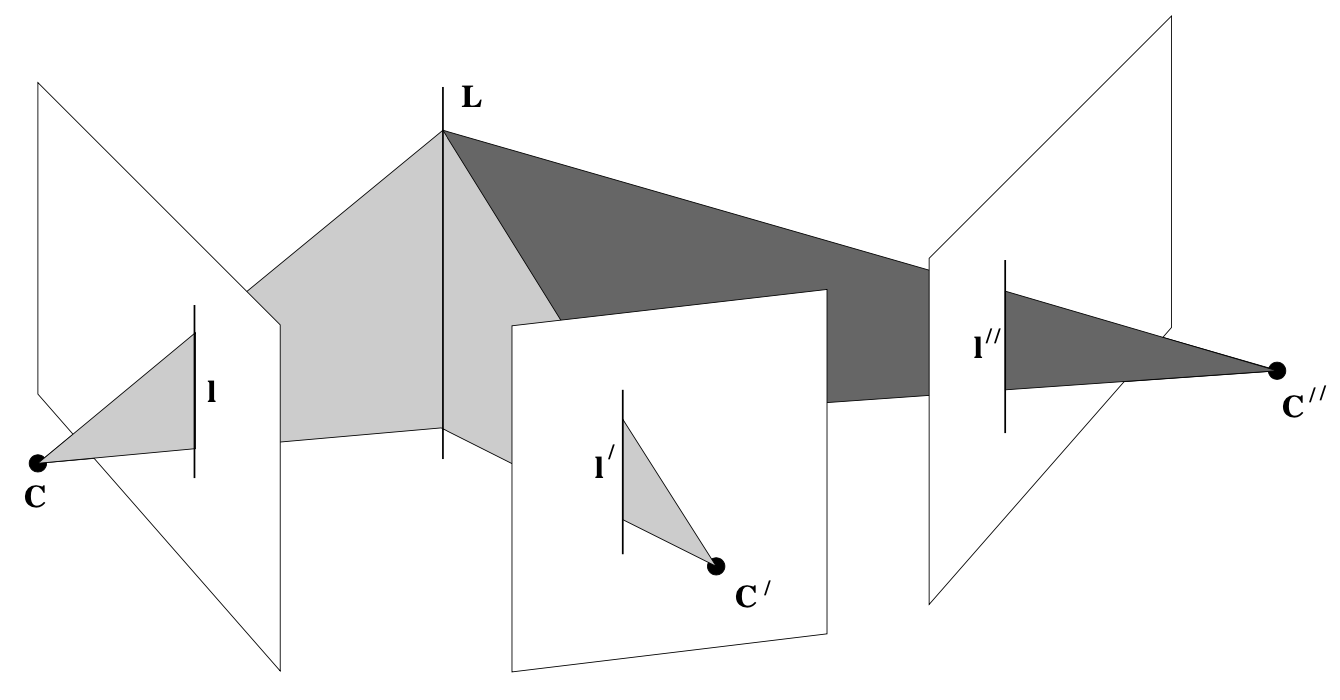
\includegraphics[width=0.5\textwidth]{Report/Figures/three-views.png}
	\caption{A line L in 3-space is imaged as the corresponding triplet \( l \leftrightarrow l' \leftrightarrow l'' \) in three views indicated by their centres, \( C \), \( C' \) , \( C'' \) , and image planes. Conversely, corresponding lines back-projected from the first, second and third images all intersect in a single 3D line in space.}
\end{figure}

Considering projective transformations, we focus on properties such as image coordinates and 3D incidence relations, which remain invariant. Each image line is projected back to a plane, with these planes constrained to intersect at the common line in 3D space. This constraint is algebraically expressed by ensuring that a specific matrix \( M = [\pi, \pi', \pi''] \) has a rank of 2. Here, \( \pi \), \( \pi' \), and \( \pi'' \) represent the back-projected planes of the image lines in each view
\begin{equation}
	\pi = P^\top l = \left( \begin{array}{c} l \\ 0 \end{array} \right) \quad
	\pi' = P'^\top l' = \left( \begin{array}{c} A^\top l' \\ a_4^\top l' \end{array} \right) \quad
	\pi'' = P''^\top l'' = \left( \begin{array}{c} B^\top l'' \\ b_4^\top l'' \end{array} \right).
\end{equation}

The latter intersection constraint induces the following incidence relation amongst the image lines
\begin{equation}
	l_i = l'^\top \bm{T}_il'',
	\label{eq:incidenceRelation}
\end{equation}

where \( \bm{T}_i = a_ib_4^\top - a_4b_i^\top \), \( i = 1, 2, 3 \). The set of three matrices \( [\bm{T}_1, \bm{T}_2, \bm{T}_3] \) constitute the \textbf{Trifocal Tensor (TFT) in matrix notation}. Hence, the incidence relation (\ref{eq:incidenceRelation}) can be expressed as
\begin{equation}
	l^\top = l'^\top [\bm{T}_1, \bm{T}_2, \bm{T}_3] l''.
	\label{eq:incidenceRelationMatrix}
\end{equation}

\subsection{Tensor Notation}
Image points and lines are represented by homogeneous column and row 3-vectors, respectively. The \( ij \)-th entry of a matrix \( A \) is denoted by \( a_i^j \), index \( i \) being the contravariant (row) index and \( j \) being the covariant (column) index. If the canonical \( 3 \times 4 \) camera matrices are \( P = [I|0] \), \( P' = [a_j^i] \), and \( P'' = [b_j^i] \), the definition of the \textbf{Trifocal Tensor (TFT) in tensor notation} becomes
\begin{equation}
	\mathbfcal{T}_i^{jk} = a_i^jb_4^k - a_4^jb_i^k.
	\label{eq:tensorDef}
\end{equation}

The placement of indices in the tensor (two contravariant and one covariant) follows the arrangement of indices on the right side of the equation. Hence, the trifocal tensor is a mixed contravariant-covariant valency 3 tensor denoted by a homogeneous array of size \( 3 \times 3 \times 3 \) (\ie, 27 elements) and possesses 18 degrees of freedom.\\

Thus, the fundamental incidence relation (\ref{eq:incidenceRelation}) is expressed as
\begin{equation}
	l_i = l'_jl''_k\mathbfcal{T}_i^{jk}.
	\label{eq:incidenceRelationTensor}
\end{equation}

\subsection{Trilinearities}\label{sec:trilinearities}
Similarly to the fundamental matrix in two-view geometry, the trifocal tensor encodes relationships between points and lines across three perspectives. These relationships are denoted as trilinearities: "tri" since every monomial in the relation involves a coordinate from each of the three image elements involved, and linear because the relations are linear in each of the algebraic entities (\ie, the three arguments of the tensor). The following equation portrays a point-point-point (P-P-P) correspondence 
\begin{equation}
	[x']_{\times} \left( \sum_{i}x^i\bm{T}_i \right) [x'']_{\times} = 0_{3 \times 3}
	\label{eq:tftTrilinearities}
\end{equation}

with \( x \), \( x' \), and \( x'' \) being the homogeneous coordinates of corresponding points in three images. However, other trilinear relations can be derived, such as L-L-L, P-L-L, P-L-P, P-P-L, and P-P-P, where P stands for point and L stands for line. These trilinearities are invariant under projective transformations, ensuring robustness across different camera configurations and scenes.\\

Among the nine scalar equations in (\ref{eq:tftTrilinearities}), only four are linearly independent. They manifest linearity with respect to the parameters of the trifocal tensor and trilinearity with respect to the image coordinates. When viewed in pairs, the incidence relationships established by the fundamental matrices for the corresponding triplet \( x \), \( x' \), and \( x'' \) consist of a group of three equations that are linear with respect to the parameters of the fundamental matrices and bilinear with respect to the image points
\begin{equation}
	x_2^\top F_{21}x_1 = 0 \quad x_3^\top F_{31}x_1 = 0 \quad x_3^\top F_{32}x_2 = 0,
\end{equation}

where the involved fundamental matrices are
\begin{equation}
	F_{21} = [a_4]_{\times}A \quad F_{31} = [b_4]_{\times}B \quad F_{32} = [b_4 - BA^{-1}a_4]_{\times}BA^{-1}.
\end{equation}

\subsection{Linear Computation}
The trifocal tensor can be derived from a linear system described by the trilinear relationships outlined in (\ref{sec:trilinearities}). Each triplet yields nine equations that are linear with respect to the tensor's parameters, yet only four of these equations are linearly independent. To solve this linear system, a minimum of seven correspondences is required, with the additional constraint \( || \mathbfcal{T} || = 1 \). If more triplets are available, a solution minimizing the algebraic error can be obtained via Singular Value Decomposition (SVD). However, the resulting trifocal tensor may not always be valid.\\

To fix this, a valid trifocal tensor can be computed through an algebraic minimization algorithm that parallels the linear process employed to find the fundamental matrix.

\begin{algorithm}[h]
		\caption{Algebraic Minimization Algorithm (Linear TFT Computation)}
		\kwObjective{Given a set of point and line correspondences in three views, compute the trifocal tensor.}
		\kwAlgorithm{
		\begin{enumerate}[label=(\roman*),leftmargin=*,rightmargin=1.5em]
        	\item From the set of point and line correspondences compute the set of equations of the form \( At = 0 \), where \( t \) is the 27-vector made up of the entries of the trifocal tensor.
        	\item Solve these equations using the least-squares solution to constrained systems, in order to find an initial estimate of the trifocal tensor \( \mathbfcal{T}_i^{jk} \).
        	\item Find the two epipoles \( e' \) and \( e'' \) from \( \mathbfcal{T}_i^{jk} \) as the common perpendicular to the left null-vectors of the three slices \( \bm{T}_i \).
        	\item Construct the \( 27 \times 18 \) matrix \( E \) such that \( t = Ea \), where a is the vector representing entries of \( a_i^j \) and \( b_i^k \), and where \( E \) espresses the linear relationship \( \mathbfcal{T}_i^{jk} = a_i^j{e''}^k - {e'}^jb_i^k \).
        	\item Minimize \( || AEa || \) subject to \( || Ea || = 1 \), . Compute the error vector \( \epsilon = AEa \).
        	\item \textbf{Iteration:} The mapping \( (e', e'') \mapsto \epsilon \) is a mapping from \( \mathbb{R}^6 \) to \( \mathbb{R}^27 \). Iterate on the last two steps with varying \( e' \) and \( e'' \) using the Levenberg-Marquardt algorithm to find the optimal \( e' \), \( e'' \) pair. Hence find the optimal \( t = Ea \) containing the entries \( \mathbfcal{T}_i^{jk} \).
    	\end{enumerate}
    }
\end{algorithm}

\subsection{Optimization}
Several potential concise descriptions of the trifocal tensor have been suggested in prior literature \cite{4-minimal-constraints-tft, 5-nonlinear-three-view-estimation, 3-tft-vs-fund, 6-nordberg-param, 7-faugeras-papadopoulo-param, 8-ponce-hebert-param, 9-ressl-param, 10-robust-param}. We've opted to concentrate on four representative ones that can be seamlessly integrated into the pose estimation procedure.

\paragraph{Ressl}
Ressl, in his thesis \cite{9-ressl-param}, introduced a minimal parameterization for the trifocal tensor, relying on algebraic constraints within correlation slices. This formulation consists of 20 parameters and 2 constraints. It enables the comprehensive characterization of the trifocal tensor for three views. The trifocal tensor, represented by the three matrices \( T_i \), can be succinctly parameterized as follows
\begin{equation}
	\bm{T}_i = [s_i, vs_i + m_ie_{31}, ws_i + n_ie_{31}]^\top,
\end{equation}

where \( s_i \in \mathbb{R}^3 \) are such that \( || (s_1 s_2 s_3) || = 1 \), \( e_{31} \in \mathbb{R} \) with \( || e_{31} || = 1 \), and \( v, w, m_i, n_i \in \mathbb{R} \).\\

This parameterization directly links to the epipoles: where \( e_{31} = b_4 \) signifies the epipole, the projection of the first camera center onto the third image, and \( e_{21} = a_4 \) is proportionate to \( (1,v,w)^\top \). Moreover, it's tied to an equivalent parameterization of three canonical projective matrices.

\paragraph{Nordberg}
Another approach to parameterize the trifocal tensor involves three \( 3 \times 3 \) orthogonal matrices, \( U \), \( V \), and \( W \), as mentioned in \cite{6-nordberg-param}. These matrices transform the original tensor into a sparse form, denoted as \( \bm{\widetilde{\mathbfcal{T}}} \), containing only 10 non-zero parameters, up to scale
\begin{equation}
	\bm{\widetilde{\mathbfcal{T}}} = \mathbfcal{T} (U \otimes V \otimes W),
\end{equation}

where the tensor operation \( \otimes \) corresponds to the matrix operation on the slices \( \widetilde{T_i} = V^\top (\sum_{m}U_{m,i}T_m) W \). The scale can be fixed by imposing \( || \bm{\widetilde{\mathbfcal{T}}} || = 1 \).\\

For canonical cameras, such orthogonal matrices can be computed as
\begin{equation}
	\begin{gathered}
		U_0 = (A^{-1}a_4, {[A^{-1}a_4]_{\times}}^2B^{-1}b_4, [A^{-1}a_4]_{\times}B^{-1}b_4)\\
		U = U_0(U_0^\top U_0)^{-\frac{1}{2}}\\
		V_0 = (a_4, [a_4]_{\times}AB^{-1}b_4, {[a_4]_{\times}}^2AB^{-1}b_4)\\
		V = V_0(V_0^\top V_0)^{-\frac{1}{2}}\\
		W_0 = (b_4, [b_4]_{\times}BA{-1}a_4, {[b_4]_{\times}}^2BA^{-1}a_4)\\
		W = W_0(W_0^\top W_0)^{-\frac{1}{2}},
	\end{gathered}
\end{equation}

and each matrix can be represented by 3 parameters, resulting in a total of 19 parameters for the trifocal tensor \( \mathbfcal{T} \), along with one constraint to determine the scale of \( \bm{\widetilde{\mathbfcal{T}}} \).\\

However, a notable drawback of this particular parameterization arises when the camera centers are collinear. In such cases, the matrices \( U_0 \), \( V_0 \), and \( W_0 \) become singular, rendering it impossible to compute orthogonal matrices from them. Consequently, this parameterization is only applicable when the camera centers are non-collinear.

\paragraph{Faugeras and Papadopoulo}
The work outlined in \cite{7-faugeras-papadopoulo-param} introduces a set of 12 algebraic equations, serving as constraints to fully define a trifocal tensor. These include three constraints of third-degree, corresponding to the slices' determinants being zero, \( |T_i| = 0 \) for \( i \in \{1, 2, 3\} \), and an additional nine constraints of sixth-degree. These sixth-degree constraints involve combinations of various determinants of the tensor's elements
\begin{equation}
	\begin{gathered}
		| \bm{T}_.^{j_1}{k_1}\bm{T}_.^{j_1}{k_2}\bm{T}_.^{j_2}{k_2} | | \bm{T}_.^{j_1}{k_1}\bm{T}_.^{j_2}{k_1}\bm{T}_.^{j_2}{k_2} | -\\
		| \bm{T}_.^{j_2}{k_1}\bm{T}_.^{j_1}{k_2}\bm{T}_.^{j_2}{k_2} | | \bm{T}_.^{j_1}{k_1}\bm{T}_.^{j_2}{k_2}\bm{T}_.^{j_1}{k_2} | = 0,
	\end{gathered}
\end{equation}

where \( j_1, j_2, k_1, k_2 \in \{1, 2, 3\} \) with \( j_1 \neq j_2 \) and \( k_1 \neq k_2 \), and where \( \bm{T}_.^{jk} \) represents the vector \( (\bm{T}_1^{jk}, \bm{T}_2^{jk}, \bm{T}_3^{jk})^\top \).\\

This collection isn't minimal because it requires just 9 constraints to fully define a valid trifocal tensor. The authors suggest a method for achieving a minimal parameterization using these constraints, which involves solving a second-degree polynomial, resulting in two potential tensors. We find it preferable to pursue constraint minimization rather than minimal parameters for a simpler implementation.

\paragraph{Ponce and Hebert \( \bm{\Pi} \) Matrices}
An alternative method of characterizing the 3-view model has been investigated in \cite{8-ponce-hebert-param}. By analyzing how three lines intersect in space, a trio of matrices has been derived, each associated with principal lines. These matrices, comprising a total of 27 parameters, impose constraints on the correspondence between three image points. Analogous to the TFT, they serve a crucial role. For a configuration involving three cameras with non-collinear centers and three image points, denoted as \( x_1 \), \( x_2 \), and \( x_3 \), there exist three \( 4 \times 3 \) matrices, denoted as \( \Pi_i = (\pi_{1i}, \pi_{2i}, \pi_{3i}, \pi_{4i})^\top \), each scalable, where \( \pi_{ii} = (0 0 0)^\top \), and they satisfy

\begin{equation}
	x_1^\top (\pi_{41}\pi_{32}\top - \pi_{31}\pi_{42}\top) x_2 = 0
	\label{eq:phConst1}
\end{equation}
\begin{equation}
	x_1^\top (\pi_{41}\pi_{23}\top - \pi_{21}\pi_{43}\top) x_3 = 0
	\label{eq:phConst2}
\end{equation}
\begin{equation}
	x_3^\top (\pi_{43}\pi_{13}\top - \pi_{12}\pi_{43}\top) x_3 = 0
	\label{eq:phConst3}
\end{equation}
\begin{equation}
	(\pi_{21}^\top x_1) (\pi_{32}^\top x_2) (\pi_{13}^\top x_3) = (\pi_{31}^\top x_1) (\pi_{12}^\top x_2) (\pi_{23}^\top x_3),
	\label{eq:phConst4}
\end{equation}

if, and only if, the \( x_i \) form a triplet of corresponding points.\\
Ponce and Hebert propose the 6 following homogeneous constraints
\begin{equation}
	\begin{gathered}
		\pi_{21}^1 = \pi_{32}^2 = \pi_{13}^3 = ,0\\
		\pi_{31}^2 = \pi_{41}^3, \quad \pi_{12}^3 = \pi_{42}^1, \quad \pi_{23}^1 = \pi_{43}^2.
	\end{gathered}
\end{equation}

This can be accomplished through a projective transformation of the space, reducing the parameters to 21. By imposing three norm constraints on the matrices, \( || \Pi_i || = 1 \), we achieve the most concise representation.\\

Analogous to the trilinearities (\ref{eq:tftTrilinearities}) in the trifocal tensor scenario, these parameters yield four equations detailing the incidence relation for image points. Equations (\ref{eq:phConst1}), (\ref{eq:phConst2}), and (\ref{eq:phConst3}) are bilinear regarding the points and are entirely analogous to the epipolar equations provided by the fundamental matrices. Equation (\ref{eq:phConst4}), however, is trilinear concerning the image points, playing a pivotal role in characterizing the correspondence of three points that fundamental matrices falter at when one point resides on the line connecting two epipoles. This underscores the geometric significance of leveraging three views instead of individual pairs in characterizing matches.\\

Much like Nordberg's parameterization of the trifocal tensor, a primary limitation of the \( \Pi \) matrices is their applicability solely to non-collinear camera centers. In instances of collinear camera centers, Ponce and Hebert also proposed equivalent matrices incorporating an additional trilinear constraint.
